%----------------------------------------------------------------------------------------
%	PACKAGES AND DOCUMENT CONFIGURATIONS
%----------------------------------------------------------------------------------------

\documentclass{article}
\usepackage{graphicx} % Required for the inclusion of images
\usepackage{subfigure} % Required for the inclusion of images
\usepackage{natbib} % Required to change bibliography style to APA
\usepackage{amsmath} % Required for some math elements 
\usepackage{listings}
\usepackage{graphicx} %插入图片的宏包
\usepackage{float} %设置图片浮动位置的宏包
\usepackage{subfigure} %插入多图时用子图显示的宏包
\usepackage{times} % Uncomment to use the Times New Roman font                     
\usepackage{lstcustom}          
%----------------------------------------------------------------------------------------
%	DOCUMENT INFORMATION
%----------------------------------------------------------------------------------------


\title{\textbf{Project 1: Optimizing the Performance of a Pipelined Processor}} % Title

\author{000, Ziqi Zhao, bugenzhao@sjtu.edu.cn \\
        001, Yimin Zhao, doctormin@sjtu.edu.cn \\ } % Author name and email

\date{\today} % Date for the report

\begin{document}

\maketitle % Insert the title, author and date

\section{Introduction}
\textbf{Part A}
\\
In part A, we write three simple assembly programs to mimic three functions in example.c. 
Based on ensuring correctness,we especially focus on the functional equivalence with the example C functions. 
By selecting and placing labels in the assembly code appropriately, the code is also very readable.\\
\textbf{Part B}
\\
In part B, we modify the HCL file of the SEQ to add a new instruction --- iaddl. 
The following is the roadmap to finish this part:
\begin{itemize}
        \item Clarify the computation process of iadd and write it down at the beginning in seq-full.hcl.
        \item Add any dependence relations of iaddl to all boosigs.
        \item Design the datapath for iaddl (generate control signals for src and dst)
\end{itemize}
\textbf{Part C}
\\
We achieve full scores in the benchmark testing \textbf{in just 2 hours}, 
but we \textbf{spent 2 more days} researching all the potential methods to optimize the performance even further. 
The following is our roadmap:
\begin{itemize}
        \item Change the order of the instruction sequence to avoid data hazard and structure hazards, which leaves $CPE = 12.96$.
        \item Beyond the changes on instructions order, we use loop unrolling to reduce the number of conditional check and registers updating, which leaves $CPE = 9.83$
        \item Use a binary search tree to find the precise remaining number of loops after several rounds of unrolling to achieve complete unrolling, which leaves $CPE = 8.95$
        \item Modify the HCL file to achieve 100\% accuracy in branch prediction for certain code pattern, which brings $CPE$ down to $7.78$.
\end{itemize}
\textbf{Contribution}
\\
\textbf{Ziqi Zhao} : Part A (coding) \& Part B (coding) \& Part C (coding \& designing) \& project report(reviewing) \\
\textbf{Yimin Zhao} : Part A (reviewing \& coding) \& Part B (reviewing) \& Part C (designing) \& project report(writing)

\section{Experiments}
\subsection{Part A}
\subsubsection{Analysis}
In this part, we are asked to implement and simulate three y86 programs. 
From a macro point of view,this part is relatively easy. 
But there are plenty of optimizations worth exploring in terms of code readability and elegance.\\
\textbf{Difficult Point} 
\begin{itemize}
        \item Always pull the correct element from the stack.
        \item Be careful to protect the callee-save register.
        \item Implement function recursion smartly.
\end{itemize}
\textbf{Core Technique}
\begin{itemize}
        \item Mimicking C functions, division of functional areas with enough and clear label.
        \item Get the fastest completion speed by coding line by line refering to C language functions
        \item Always draw a picture of the stack to ensure the correctness of fetching a variable.
\end{itemize}

\subsubsection{Code}
\begin{center}
        \textbf{sum.ys}
\end{center}

\begin{lstlisting}
# 518030910211 ZiqiZhao
# 518030910188 YiminZhao

# Set up stack
        .pos    0
        irmovl  stack,  %esp
        rrmovl  %esp,   %ebp
        pushl   %edx            # save %edx
        irmovl  ele1,   %eax
        pushl   %eax
        call    sum_list
        popl    %edx            # flatten the stack for ele1
        popl    %edx            # restore %edx
        halt

# Sample linked list 
.align 4
ele1:
        .long   0x00a
        .long   ele2
ele2:
        .long   0x0b0
        .long   ele3
ele3:
        .long   0xc00
        .long   0

# sum_list func
sum_list:
        pushl   %ebp            # enter
        pushl   %ecx            # save %ecx
        rrmovl  %esp,   %ebp
        xorl    %eax,   %eax    # clear %eax
        mrmovl  12(%ebp),%edx   # get ls
        jmp     test
loop:
        mrmovl  (%edx), %ecx
        addl    %ecx,   %eax
        mrmovl  4(%edx),%edx
test:
        andl    %edx,   %edx
        jne     loop            # %edx != 0
return:
        rrmovl  %ebp,   %esp    # leave
        popl    %ecx
        popl    %ebp
        ret

# Stack 
        .pos    0x400
stack:
\end{lstlisting}
\pagebreak
\begin{center}
        \textbf{rsum.ys}
\end{center}
\begin{lstlisting}
# 518030910211 ZiqiZhao
# 518030910188 YiminZhao

# Set up stack
    .pos    0
    irmovl  stack, %esp
    rrmovl  %esp, %ebp
    pushl   %edx
    irmovl  ele1, %eax
    pushl   %eax
    call    rsum_list
    popl    %edx           # eat ele1
    popl    %edx           # restore %edx
    halt

# Sample linked list 
.align 4
ele1:
    .long   0x00a
    .long   ele2
ele2:
    .long   0x0b0
    .long   ele3
ele3:
    .long   0xc00
    .long   0

# rsum_list func
rsum_list:
    pushl   %ebp            # enter
    rrmovl  %esp, %ebp
    xorl    %eax, %eax
    mrmovl  8(%ebp), %edx   # get ls
    andl    %edx, %edx
    je      return          # ls == NULL
do:
    pushl   %ebx            # save %ebx
    mrmovl  (%edx), %ebx    # mov ls->val to %ebx
    mrmovl  4(%edx), %eax
    pushl   %eax            # push ls->next
    call    rsum_list
    addl    %ebx, %eax      # ret = val + ret
    popl    %edx            # eat para
    popl    %ebx            # restore %ebx
return:
    rrmovl  %ebp, %esp      # leave
    popl    %ebp
    ret


# Stack 
    .pos    0x400
stack:
\end{lstlisting}
\begin{center}
        \textbf{copy.ys}
\end{center}
\begin{lstlisting}
# 518030910211 ZiqiZhao
# 518030910188 Yimin Zhao

# Set up stack
    .pos    0
    irmovl  stack, %esp
    rrmovl  %esp, %ebp
    irmovl  $3, %eax
    pushl   %eax
    irmovl  src, %eax
    pushl   %eax
    irmovl  dest, %eax
    pushl   %eax
    call    copy_block
    halt
.align 4
# Source block
src:
    .long 0x00a
    .long 0x0b0
    .long 0xc00

# Destination block
dest:
    .long 0x111
    .long 0x222
    .long 0x333

copy_block:
    pushl   %ebp
    rrmovl  %esp, %ebp
    pushl   %ecx
    pushl   %edx
    pushl   %edi
    irmovl  $0, %eax         # %eax = result = 0
    mrmovl  16(%ebp), %ecx   # %ecx = len
    mrmovl  12(%ebp), %edx   # %edx = src
    mrmovl  8(%ebp), %edi    # %edi = dest
    jmp     while_loop

while_loop:
    andl    %ecx, %ecx       # check if %ecx == 0?
    jle     return           # if so, jump to "return"
    mrmovl  (%edx), %esi     # %esi = val = *src
    irmovl  $4, %ebx         # %ebx = 4
    addl    %ebx, %edx       # src++
    rmmovl  %esi, (%edi)     # *dest = val
    addl    %ebx, %edi       # dest++
    xorl    %esi, %eax
    irmovl  $-1, %ebx
    addl    %ebx, %ecx       # len--
    jmp     while_loop

return:
    popl    %edi
    popl    %edx
    popl    %ecx
    rrmovl  %ebp, %esp
    popl    %ebp
    ret
# Stack 
    .pos    0x400
stack:
\end{lstlisting}
\pagebreak
\subsubsection{Evaluation}
\textbf{sum.ys}\\

\begin{figure}[H] %H为当前位置,!htb为忽略美学标准,htbp为浮动图形
        \centering %图片居中
        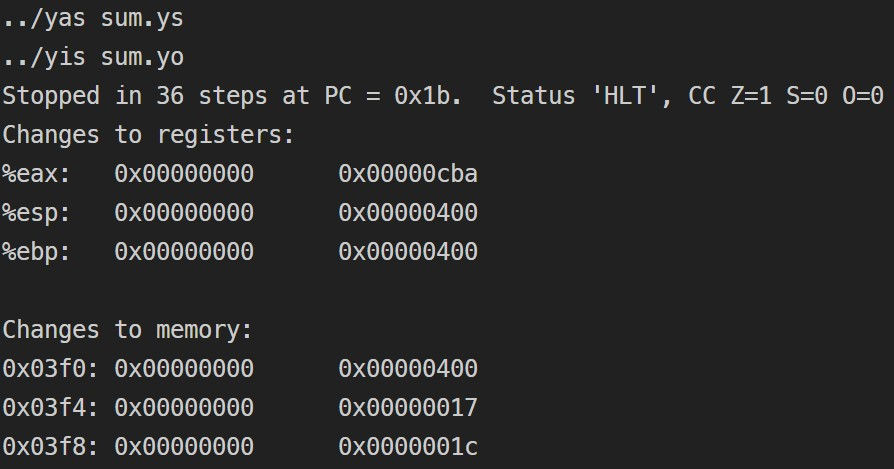
\includegraphics[width=0.7\textwidth]{partA-sum.jpg} %插入图片,[]中设置图片大小,{}中是图片文件名
        \caption{partA-sum.ys} %最终文档中希望显示的图片标题
        \label{Fig.partA-sum} %用于文内引用的标签
\end{figure}
\begin{itemize}
        \item The \%eax register has the correct value which is the return value of the function---$0xcba$.
        \item The memory is not corrupted since all the modifications locate at the stack whose starting addresss is set to be $0x400$.
\end{itemize}
\textbf{rsum.ys}\\

\begin{figure}[H] %H为当前位置,!htb为忽略美学标准,htbp为浮动图形
        \centering %图片居中
        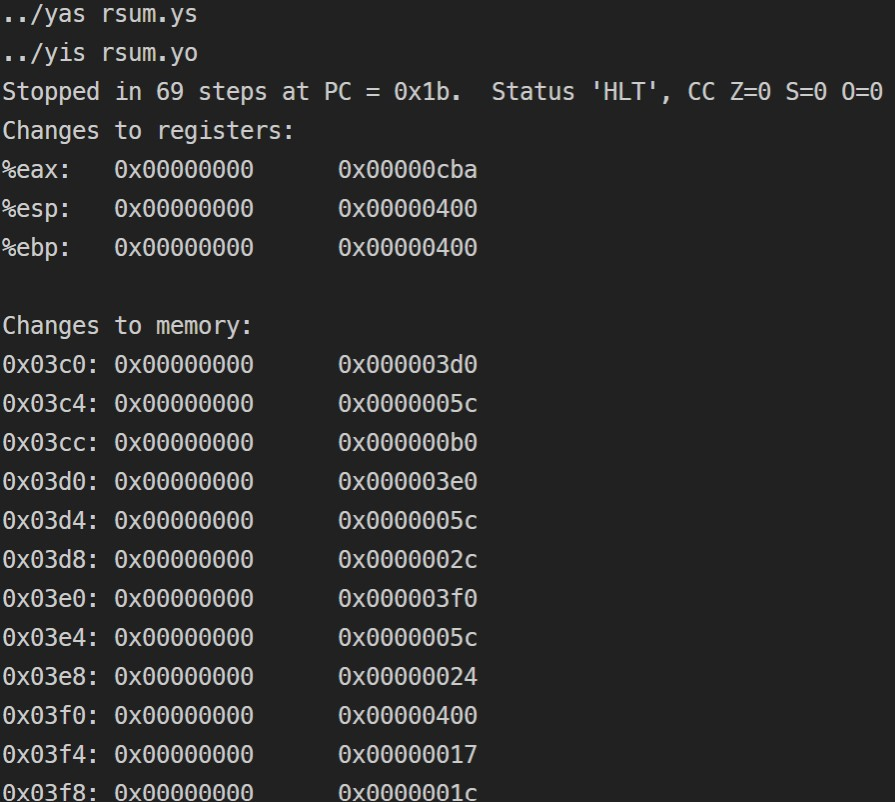
\includegraphics[width=0.7\textwidth]{partA-rsum.jpg} %插入图片,[]中设置图片大小,{}中是图片文件名
        \caption{partA-rsum.ys} %最终文档中希望显示的图片标题
        \label{Fig.partA-rsum} %用于文内引用的标签
\end{figure}

\begin{itemize}
        \item The \%eax register has the correct value which is the return value of the function---$0xcba$.
        \item The memory is not corrupted since all the modifications locate at the stack whose starting addresss is set to be $0x400$.
\end{itemize}

\textbf{copy.ys}\\

\begin{figure}[H] %H为当前位置,!htb为忽略美学标准,htbp为浮动图形
        \centering %图片居中
        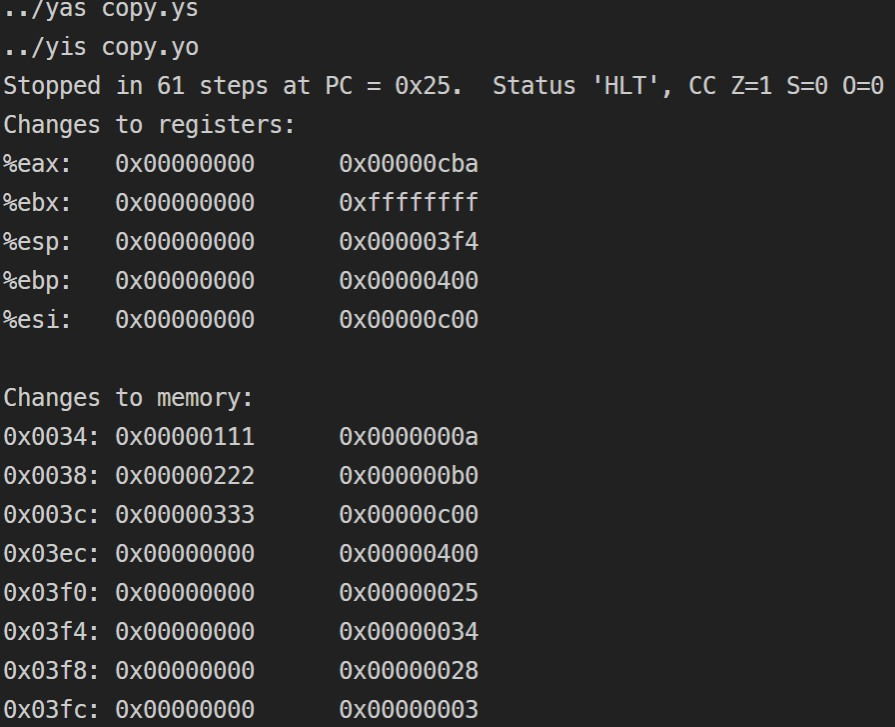
\includegraphics[width=0.7\textwidth]{partA-copy.jpg} %插入图片,[]中设置图片大小,{}中是图片文件名
        \caption{partA-copy.ys} %最终文档中希望显示的图片标题
        \label{Fig.partA-copy} %用于文内引用的标签
\end{figure}

\begin{itemize}
        \item The \%eax register has the correct value which is the return value of the function---$0xcba$.
        \item Values are written into the memory correctly as shown in the first three rows in the "Changes to memory" part in Figure 3
        \item The memory is not corrupted since all the modifications other than 3 source values locate at the stack whose starting addresss is set to be $0x400$.
\end{itemize}

\subsection{Part B}

\subsubsection{Analysis}
In part B, we are asked to extend the SEQ processor to support instruction "iaddl" by modifying SEQ-full.hcl.
Once we understand the processing logic and HCL syntax of the y86 seq processor, the problem becomes very simple.
We can do it in five minutes because all we need to do is change the followings in the HCL
\begin{itemize}
        \item Add "IIADDL" in the choices region of (bool) instr\_valid since iaddl is a valid instruction.
        \item Add "IIADDL" in the choices region of (bool) need\_regid since iaddl operation involves one register.
        \item Add "IIADDL" in the choices region of (bool) need\_valC since iaddl operation involves one constend(represented by valC in the circult of y86 SEQ).
        \item Add "IIADDL" in the choices region of (bool) set\_cc since iaddl operation involves ALU operation which will set flags.
        \item When icode is IIADDL, alufun will be ALUADD since the operation is "adding" the constand to rB.
        \item When icode is IIADDL, srcB is from rB since the second operand of iaddl is a register.
        \item When icode is IIADDL, dstE (where the result from ALU is passed towards) is rB since "iaddl constant, rB" means rB += constant (rB is updated). 
        \item When icode is IIADDL, aluA (the first op) is valC (the constant in the instruction) since "iaddl constant, rB" means the first op is the constant (valC).
        \item When icode is IIADDL, aluB (the second op) is valB (the value of the second register that is read) for the same reason above.
\end{itemize}
[In this part, you should give an overall analysis for the task, like difficult point, core technique and so on.]

\subsubsection{Code}
\begin{center}
        \textbf{Modifications in SEQ-full.hcl}
\end{center}
\begin{lstlisting}
--------------------------------------------------------------------
bool instr_valid = icode in 
{ INOP, IHALT, IRRMOVL, IIRMOVL, IRMMOVL, IMRMOVL,
       IOPL, IJXX, ICALL, IRET, IPUSHL, IPOPL, IIADDL };
--------------------------------------------------------------------
# Does fetched instruction require a regid byte?
bool need_regids =
        icode in { IRRMOVL, IOPL, IPUSHL, IPOPL, 
                IIRMOVL, IRMMOVL, IMRMOVL, IIADDL };
--------------------------------------------------------------------
# Does fetched instruction require a constant word?
bool need_valC =
        icode in { IIRMOVL, IRMMOVL, IMRMOVL, IJXX, ICALL, IIADDL };
--------------------------------------------------------------------
## What register should be used as the B source?
int srcB = [
        icode in { IOPL, IRMMOVL, IMRMOVL, IIADDL  } : rB;
        icode in { IPUSHL, IPOPL, ICALL, IRET } : RESP;
        1 : RNONE;  # Don't need register
];
--------------------------------------------------------------------
## What register should be used as the E destination?
int dstE = [
        icode in { IRRMOVL } && Cnd : rB;
        icode in { IIRMOVL, IOPL, IIADDL } : rB;
        icode in { IPUSHL, IPOPL, ICALL, IRET } : RESP;
        1 : RNONE;  # Don't write any register
];
--------------------------------------------------------------------
## Select input A to ALU
int aluA = [
        icode in { IRRMOVL, IOPL } : valA;
        icode in { IIRMOVL, IRMMOVL, IMRMOVL, IIADDL } : valC;
        icode in { ICALL, IPUSHL } : -4;
        icode in { IRET, IPOPL } : 4;
        # Other instructions don't need ALU
];
--------------------------------------------------------------------
## Select input B to ALU
int aluB = [
        icode in { IRMMOVL, IMRMOVL, IOPL, ICALL, 
                IPUSHL, IRET, IPOPL, IIADDL } : valB;
        icode in { IRRMOVL, IIRMOVL } : 0;
        # Other instructions don't need ALU
];
--------------------------------------------------------------------
## Set the ALU function
int alufun = [
        icode == IOPL : ifun;
        icode == IIADDL : ALUADD;
        1 : ALUADD;
];
--------------------------------------------------------------------
## Should the condition codes be updated?
bool set_cc = icode in { IOPL, IIADDL };
--------------------------------------------------------------------
\end{lstlisting}
\subsubsection{Evaluation}
\begin{figure}[H] %H为当前位置,!htb为忽略美学标准,htbp为浮动图形
        \centering %图片居中
        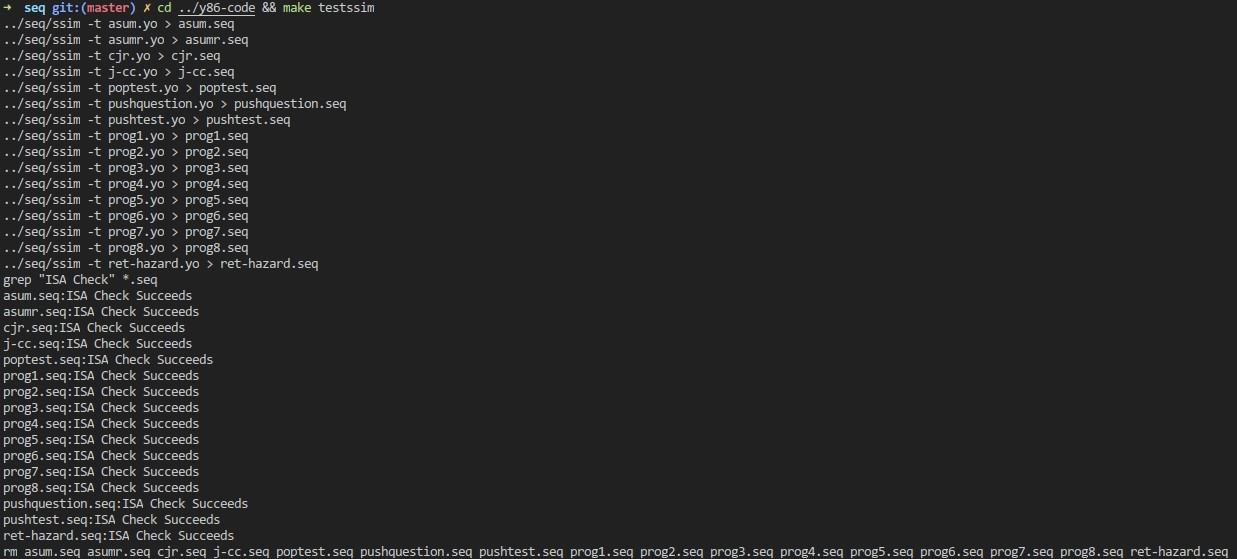
\includegraphics[width=1.0\textwidth]{partB-benchmark.jpg} %插入图片,[]中设置图片大小,{}中是图片文件名
        \caption{part B benchmark test} %最终文档中希望显示的图片标题
        \label{Fig.partB-benchmark} %用于文内引用的标签
\end{figure}
\begin{figure}[H] %H为当前位置,!htb为忽略美学标准,htbp为浮动图形
        \centering %图片居中
        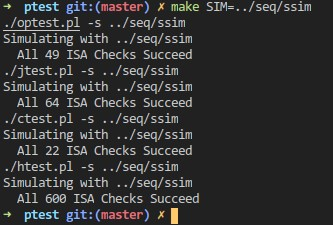
\includegraphics[width=0.6\textwidth]{partB-regression-test.jpg} %插入图片,[]中设置图片大小,{}中是图片文件名
        \caption{part B regression test} %最终文档中希望显示的图片标题
        \label{Fig.partB-regression} %用于文内引用的标签
\end{figure}
\begin{figure}[H] %H为当前位置,!htb为忽略美学标准,htbp为浮动图形
        \centering %图片居中
        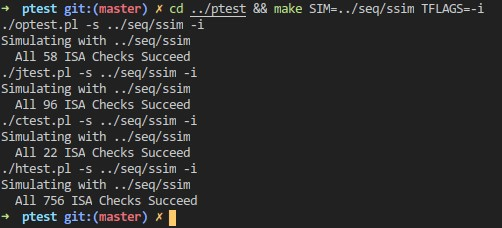
\includegraphics[width=0.6\textwidth]{partB-test-iaddl.jpg} %插入图片,[]中设置图片大小,{}中是图片文件名
        \caption{part B iaddl test} %最终文档中希望显示的图片标题
        \label{Fig.partB-iaddl} %用于文内引用的标签
\end{figure}
\subsection{Part C}
\subsubsection{Analysis}
In this part, we were asked to speed up the program ncopy.ys 
as much as possible by modifying the ncopy.ys and HCL.
The following is our roadmap:\\
\\
\textbf{Avoid Load and Use: CPI $\rightarrow$ 12.96} \\
For the pipeline design in CS:APP 2e, "load and use" or "mrmovl" then "rmmovl" will cause penalty,
which must be avoided to improve the performance. On the one hand, we rearranged the order of 
instructions to avoid stalling as much as possible. On the other hand, we use two registers to store 
the variable "val" , loading them separately and ahead of time.\\
\\
\textbf{10-way Loop Unrolling:  CPI $\rightarrow$ 9.83} \\
There's much overhead in testing and updating procedure of loops, and one way to minimize it is to 
perform a technique named "loop unrolling". That is, we do multiple loops and update the relevant 
data at once, to reduce the number of times we execute the 'add' and 'jxx' instructions. \\
\\
\textbf{Search Tree for Remaining Elements:  CPI $\rightarrow$ 8.95} \\
For large inputs, the more ways we unroll the loops, the better the program performs. However, for 
small inputs, it is important to choose a good method to process the remaining elements. The simplest 
way is to write another loop for them, but a much better way is to totally unroll the code, that is, 
jump to different position for different number of remaining ones. Since Y86 does not support relative 
jump instruction, we designed a search tree to get the correct jump destination for each possibility.
\\
\\
--------------------------------------------------------------------------------------------------------\\
The above optimization took us two hours, so far we have reached full marks
But \textbf{can it be even faster} ?
We spent another two days poring over the implementation logic and HCL and other files of the y86 pipeline. 
And it finally gets us here:\\
--------------------------------------------------------------------------------------------------------\\
\\
\textbf{Optimized for Our Branch Prediction Design: CPI $\rightarrow$ 7.78} \\
For this program, a significant performance factor is the branch prediction failure for count++. In 
"pipe-zzcc.hcl", we made a special optimization for the situation like this:\\
\begin{tabular}{|c|c|c|c|}
        \hline Instruction:&any instruction&non-alu instruction&jxx\\
        \hline Stages:&EX&ID&IF\\
        \hline
\end{tabular}
\\
Note that in this case, we can forward the conditions from EX stage to IF and predict the branch with 100\% accuracy. 
Thus, we optimized the program to ensure that there were as many of these patterns as 
possible and took much advantage of it, which leads to an average CPE of 7.78.
\subsubsection{Code}
\begin{center}
        \textbf{-----10-Way Loop Unrolling-----}\\
\end{center}
\begin{lstlisting}
# Entry
	iaddl $-9, %edx		# len -= 9, i.e., initial_len <= 9?
	irmovl $0, %eax		# count = 0
	jle Remaining		# if so, goto Remaining

# Loop unrolling part
Loop0:	
	mrmovl (%ebx), %esi	# valA = src[0]
	mrmovl 4(%ebx), %edi	# valB = src[1]
	andl %esi, %esi		# valA <= 0?
	rmmovl %esi, (%ecx)	# dst[0] = valA
	jle Loop1		# if so, goto next loop
	iaddl $1, %eax		# count++
Loop1:	
	mrmovl 8(%ebx), %esi	# valA = src[2]
	andl %edi, %edi		# valB <= 0?
	rmmovl %edi, 4(%ecx)	# dst[1] = valB
	jle Loop2		# if so, goto next loop
	iaddl $1, %eax		# count++
Loop2:
	mrmovl 12(%ebx), %edi	# valB = src[3]
	andl %esi, %esi		# valA <= 0?
	rmmovl %esi, 8(%ecx)	# dst[2] = valA
	jle Loop3		# if so, goto next loop
	iaddl $1, %eax		# count++
Loop3:	
	mrmovl 16(%ebx), %esi	# valA = src[4]
	andl %edi, %edi		# valB <= 0?
	rmmovl %edi, 12(%ecx)	# dst[3] = valB
	jle Loop4		# if so, goto next loop
	iaddl $1, %eax		# count++
Loop4:
	mrmovl 20(%ebx), %edi	# valB = src[5]
	andl %esi, %esi		# valA <= 0?
	rmmovl %esi, 16(%ecx)	# dst[4] = valA
	jle Loop5		# if so, goto next loop
	iaddl $1, %eax		# count++
Loop5:	
	mrmovl 24(%ebx), %esi	# valA = src[6]
	andl %edi, %edi		# valB <= 0?
	rmmovl %edi, 20(%ecx)	# dst[5] = valB
	jle Loop6		# if so, goto next loop
	iaddl $1, %eax		# count++
Loop6:
	mrmovl 28(%ebx), %edi	# valB = src[7]
	andl %esi, %esi		# valA <= 0?
	rmmovl %esi, 24(%ecx)	# dst[6] = valA
	jle Loop7		# if so, goto next loop
	iaddl $1, %eax		# count++
Loop7:	
	mrmovl 32(%ebx), %esi	# valA = src[8]
	andl %edi, %edi		# valB <= 0?
	rmmovl %edi, 28(%ecx)	# dst[7] = valB
	jle Loop8		# if so, goto next loop
	iaddl $1, %eax		# count++
Loop8:
	mrmovl 36(%ebx), %edi	# valB = src[9]
	andl %esi, %esi		# valA <= 0?
	rmmovl %esi, 32(%ecx)	# dst[8] = valA
	jle Loop9		# if so, goto next loop
	iaddl $1, %eax		# count++
Loop9:
	andl %edi, %edi		# valB <= 0?
	rmmovl %edi, 36(%ecx)	# dst[9] = valB
	jle LoopEnd		# if so, goto loop end
	iaddl $1, %eax
LoopEnd:
	iaddl $40, %ecx		# dst += 10 * 4
	iaddl $40, %ebx		# src += 10 * 4
	iaddl $-10, %edx	# len -= 10
	jg Loop0		# if so, goto Loop0
                                # else, goto process remaining elements
\end{lstlisting}

\begin{center}
        \textbf{-----Binary Search Tree for Finding the Number of Remaining Loops-----}\\
\end{center}
\begin{lstlisting}
# The following block is a binary search tree to 
# find the number of remaining loops 
# (which must be less than 10) at minimal cost
Remaining:
	iaddl $6, %edx		# [-9,0] -> [-3,6]	(+3)
RemTest:
	irmovl $0, %esi
	jg RemTestR
	je Rem3
RemTestL:
	iaddl $2, %edx		# [-3,-1] -> [-1,1]	(+1)
	je Rem1
	jg Rem2
	jmp Done		# -1 + 1 = 0
RemTestR:
	iaddl $-3, %edx		# [1,6] -> [-2,3]	(+6)
	jg RemTestRR
	je Rem6
RemTestRL:
	iaddl $1, %edx		# [-2,-1] -> [-1,0]	(+5)
	jl Rem4
	je Rem5
RemTestRR:
	iaddl $-2, %edx		# [1,3] -> [-1,1]	(+8)
	jl Rem7
	je Rem8
\end{lstlisting}

\begin{center}
        \textbf{-----Unrolling of Remaining Loops-----}\\
\end{center}
\begin{lstlisting}
Rem9:
	mrmovl 32(%ebx), %esi	# valA = src[8]
	rmmovl %esi, 32(%ecx)	# dst[8] = valA
Rem8:	# Note that %esi == 0, directly jumping here
	#  implies that RemXb will performs correctly.
	andl %esi, %esi		# valA <= 0?
	mrmovl 28(%ebx), %esi	# valA = src[7]
	jle Rem8b		# if so, goto Rem8b
	iaddl $1, %eax		# count++
Rem8b:	rmmovl %esi, 28(%ecx)	# dst[7] = valA
Rem7:	
	andl %esi, %esi		# valA <= 0?
	mrmovl 24(%ebx), %esi	# valA = src[6]
	jle Rem7b		# if so, goto Rem7b
	iaddl $1, %eax		# count++
Rem7b:	rmmovl %esi, 24(%ecx)	# dst[6] = valA
Rem6:	
	andl %esi, %esi		# valA <= 0?
	mrmovl 20(%ebx), %esi	# valA = src[5]
	jle Rem6b		# if so, goto Rem6b
	iaddl $1, %eax		# count++
Rem6b:	rmmovl %esi, 20(%ecx)	# dst[5] = valA
Rem5:	
	andl %esi, %esi		# valA <= 0?
	mrmovl 16(%ebx), %esi	# valA = src[4]
	jle Rem5b		# if so, goto Rem5b
	iaddl $1, %eax		# count++
Rem5b:	rmmovl %esi, 16(%ecx)	# dst[4] = valA
Rem4:	
	andl %esi, %esi		# valA <= 0?
	mrmovl 12(%ebx), %esi	# valA = src[3]
	jle Rem4b		# if so, goto Rem4b
	iaddl $1, %eax		# count++
Rem4b:	rmmovl %esi, 12(%ecx)	# dst[3] = valA
Rem3:	
	andl %esi, %esi		# valA <= 0?
	mrmovl 8(%ebx), %esi	# valA = src[2]
	jle Rem3b		# if so, goto Rem3b
	iaddl $1, %eax		# count++
Rem3b:	rmmovl %esi, 8(%ecx)	# dst[2] = valA
Rem2:	
	andl %esi, %esi		# valA <= 0?
	mrmovl 4(%ebx), %esi	# valA = src[1]
	jle Rem2b		# if so, goto Rem2b
	iaddl $1, %eax		# count++
Rem2b:	rmmovl %esi, 4(%ecx)	# dst[1] = valA
Rem1:	
	andl %esi, %esi		# valA <= 0?
	mrmovl (%ebx), %esi	# valA = src[0]
	jle Rem1b		# if so, goto Rem1b
	iaddl $1, %eax		# count++
Rem1b:	
	andl %esi, %esi		# valA <= 0?
	rmmovl %esi, (%ecx)	# dst[0] = valA
	jle Done		# if so, goto Done
        iaddl $1, %eax		# count++
        
\end{lstlisting}

\begin{center}
        \textbf{-----Modification to hcl (all in pipe-zzcc.hcl)-----}\\
\end{center}
\begin{lstlisting} 
---------------------add following definition-----------------------
quote 'int gen_aluA();'			# Declaration of gen_aluA
quote 'int gen_aluB();'			# Declaration of gen_aluB

# For JXX in ID and ALU in EX, check the cc generated by ALU
# Note that the simulator do not generate `cc_in` correctly
boolsig f_cnd_alu 
        'cond_holds(compute_cc(id_ex_curr->ifun, 
                        gen_aluA(), gen_aluB()), 
                        if_id_next->ifun)'

# For JXX in ID and non-ALU in EX, check the cc register
boolsig f_cnd_other 'cond_holds(cc, if_id_next->ifun)'
-------------------------modify f_predPC----------------------------
# Predict next value of PC
int f_predPC = [
	f_icode == ICALL : f_valC;
	f_icode == IJXX && f_ifun == UNCOND : f_valC;

	# Decode stage is ALU and will set CC -> always taken by default
	f_icode == IJXX && (D_icode in {IOPL, IIADDL}): f_valC;

	# Decode stage is not ALU
	 # Execute stage is ALU -> compute CC
        f_icode == IJXX && (E_icode in {IOPL, IIADDL}) && 
        !f_cnd_alu : f_valP;

	 # Execute stage is not ALU -> check cc -> ZF SF OF
        f_icode == IJXX && !(E_icode in {IOPL, IIADDL}) && 
        !f_cnd_other : f_valP;
        # Other JXX
	f_icode == IJXX : f_valC;

	# Otherwise
	1 : f_valP;
];
---------------add conditions to D_Bubble & E_BUbble----------------
bool D_bubble =
	# Mispredicted branch taken
        (E_icode == IJXX && E_ifun != UNCOND && 
        (M_icode in {IOPL, IIADDL}) && !e_Cnd) ||
	# Stalling at fetch while ret passes through pipeline
	# but not condition for a load/use hazard
        !(E_icode in { IMRMOVL, IPOPL } 
        && E_dstM in { d_srcA, d_srcB }) 
        && IRET in { D_icode, E_icode, M_icode };

# Should I stall or inject a bubble into Pipeline Register E?
# At most one of these can be true.
bool E_stall = 0;
bool E_bubble =
	# Mispredicted branch taken
        (E_icode == IJXX && E_ifun != UNCOND && 
        (M_icode in {IOPL, IIADDL}) && !e_Cnd) ||
	# Conditions for a load/use hazard
	E_icode in { IMRMOVL, IPOPL } &&
	 E_dstM in { d_srcA, d_srcB};
\end{lstlisting}
\subsubsection{Evaluation}
\begin{figure}[H] %H为当前位置,!htb为忽略美学标准,htbp为浮动图形
        \centering %图片居中
        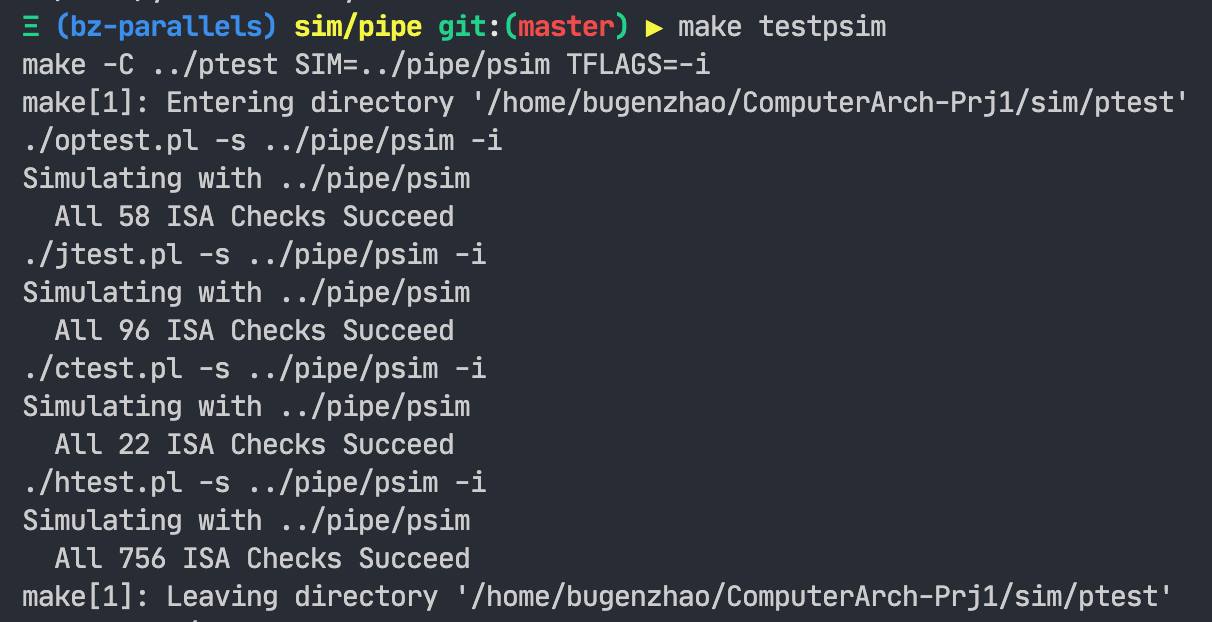
\includegraphics[width=0.7\textwidth]{partC-regression-test.png} %插入图片,[]中设置图片大小,{}中是图片文件名
        \caption{partC regression test} %最终文档中希望显示的图片标题
        \label{Fig.partC-regression} %用于文内引用的标签
\end{figure}
\begin{figure}[H] %H为当前位置,!htb为忽略美学标准,htbp为浮动图形
        \centering %图片居中
        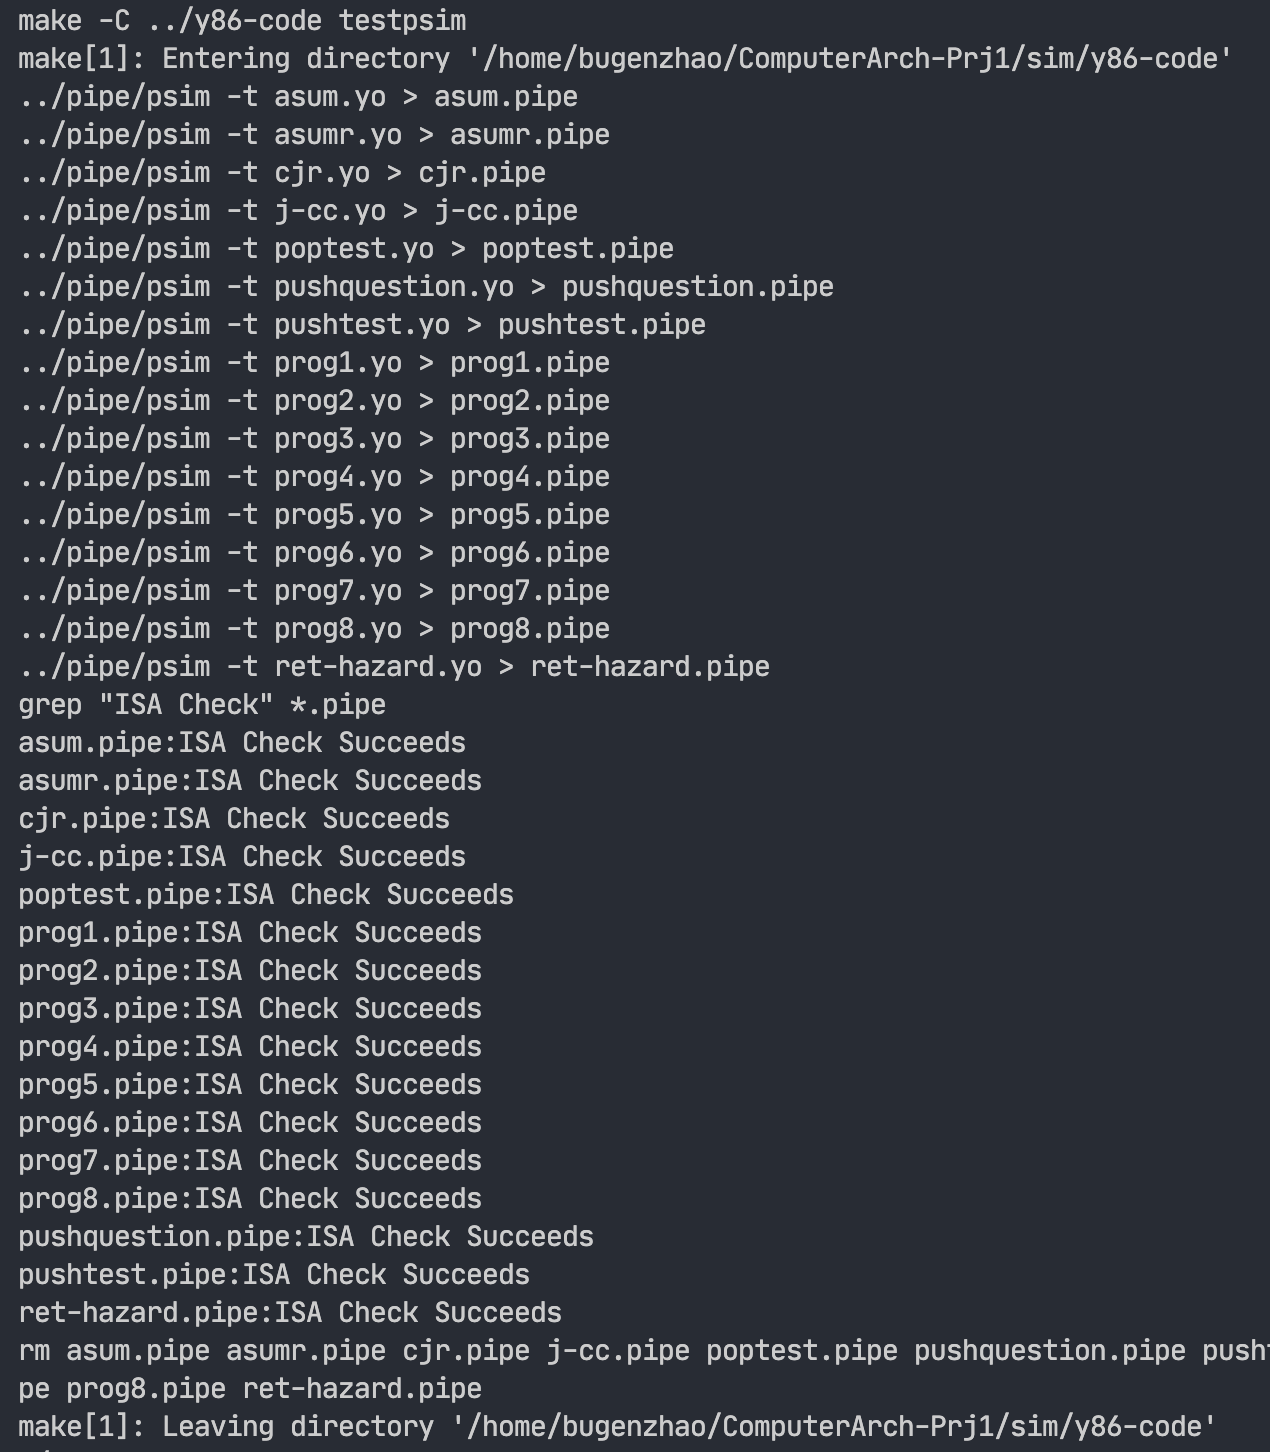
\includegraphics[width=0.7\textwidth]{partC-test2.png} %插入图片,[]中设置图片大小,{}中是图片文件名
        \caption{partC benchmark test} %最终文档中希望显示的图片标题
        \label{Fig.partC-benchmark} %用于文内引用的标签
\end{figure}
\begin{figure}[H] %H为当前位置,!htb为忽略美学标准,htbp为浮动图形
        \centering %图片居中
        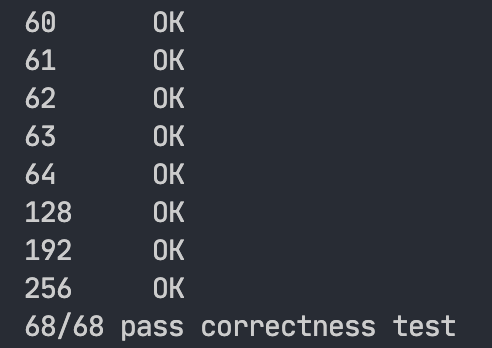
\includegraphics[width=0.4\textwidth]{partC-correctness-test.png} %插入图片,[]中设置图片大小,{}中是图片文件名
        \caption{partC correctness test} %最终文档中希望显示的图片标题
        \label{Fig.partC-correctness} %用于文内引用的标签
\end{figure}
\begin{figure}[H] %H为当前位置,!htb为忽略美学标准,htbp为浮动图形
        \centering %图片居中
        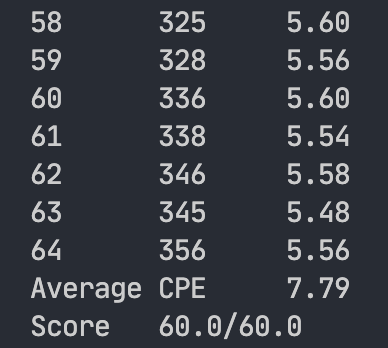
\includegraphics[width=0.4\textwidth]{partC-CPE-test.png} %插入图片,[]中设置图片大小,{}中是图片文件名
        \caption{partC CPE test} %最终文档中希望显示的图片标题
        \label{Fig.partC-CPE} %用于文内引用的标签
\end{figure}
\section{Conclusion}
In this project, we completed the tasks of three parts, 
which were gradually developed. The first part made us familiar with y86 assembly syntax, 
the second part made us familiar with y86 SEQ circuit logic, and the third part encouraged us to transform assembly code and y86 pipeline circuit logic
The following is a summary of the completion of the three parts:\\
\textbf{Part A}
\begin{itemize}
        \item We write assembly code for three simple functions.
        \item We take care to protect the stack and registers.
        \item We focus on the readability and functional equivalence of the code.
\end{itemize}
\textbf{Part B}
\begin{itemize}
        \item We modify SEQ-full.hcl to add an intruction: iaddl.
\end{itemize}
\textbf{Part C}
\begin{itemize}
        \item We reorder the instructions to avoid hazards.
        \item We do 10-way loop unrolling to speed up the while loop.
        \item We create a binary search tree to find the number of remaining loops at the minimal cost and then completely unroll the loops.
        \item We modify the HCL file of the pipeline to optimize the branch prediction,  achieving 100\% accuracy for a certain code mode (non-ALU followed by jxx).
\end{itemize}
\subsection{Problems}
We only meet problems in Part C. They are two unsuccessful attempts to modify the pipeline logic to lift accuracy of branch prediction to 100\%.
Based on attempt 2, we have made some small changes to achieve the goal, which is explained in detail in \textbf{3.2 achievement}.
\subsubsection{Attempt 1}
In this attempt, we look at a particular code distribution, 
which is "andl op1, op2 $\rightarrow$ JXX des"(because in our code, there are a lot of this kind of code distributions). 
We hope that the branch prediction of JXX under this distribution can reach 100\% accuracy.
The logic is shown in Figure 11:
\begin{figure}[H] %H为当前位置,!htb为忽略美学标准,htbp为浮动图形
        \centering %图片居中
        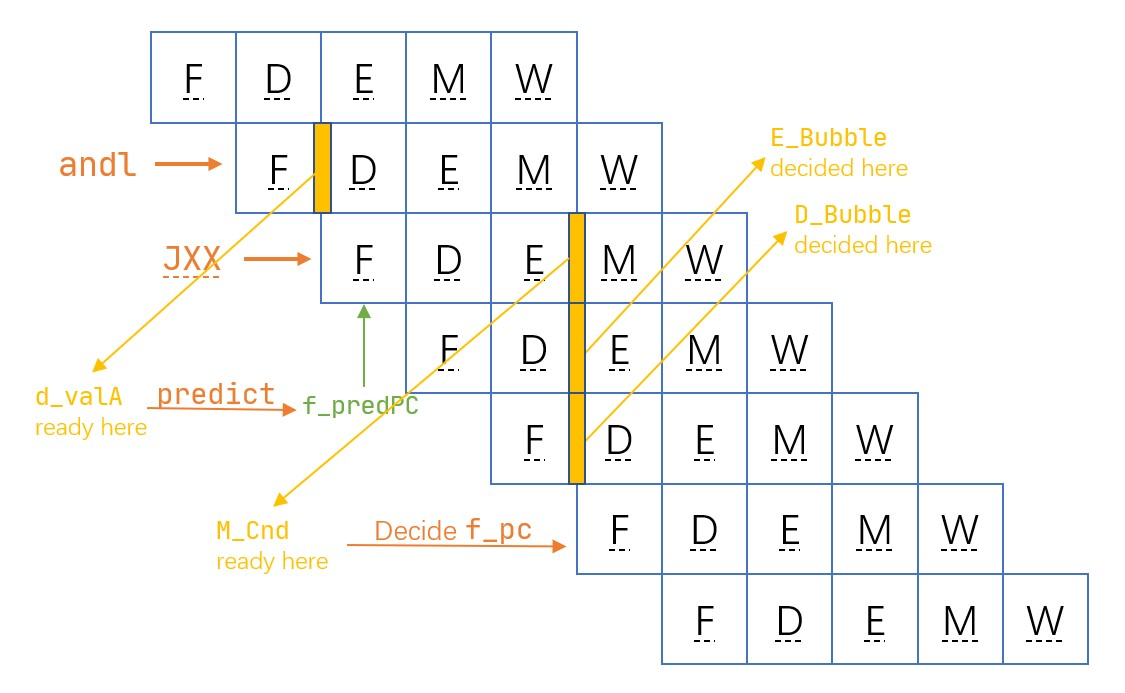
\includegraphics[width=0.7\textwidth]{partC-attempt1.jpg} %插入图片,[]中设置图片大小,{}中是图片文件名
        \caption{partC attempt1} %最终文档中希望显示的图片标题
        \label{Fig.partC-correctness} %用于文内引用的标签
\end{figure}
Basically, it means that when we detect a JXX after an andl, 
we will do branch prediction according to the value of the first op of "andl". 
Because in our ncopy.ys, there are a lot of this kind of codes:
\begin{figure}[H] %H为当前位置,!htb为忽略美学标准,htbp为浮动图形
        \centering %图片居中
        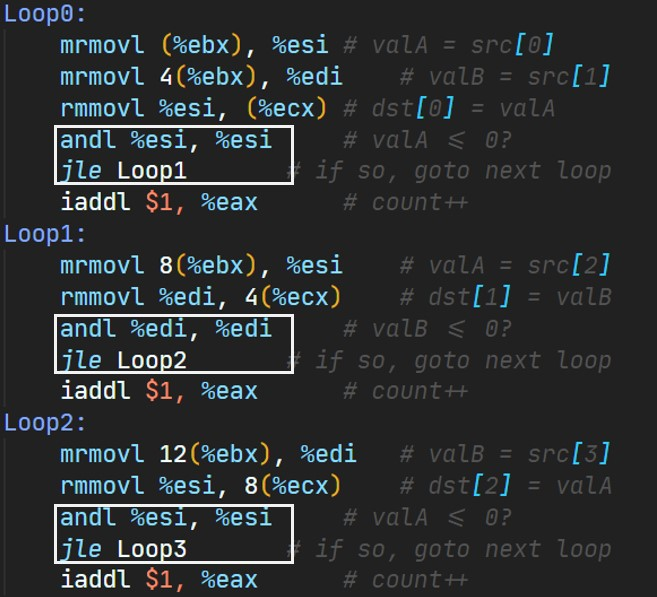
\includegraphics[width=0.5\textwidth]{partC-loop-demo.jpg} %插入图片,[]中设置图片大小,{}中是图片文件名
        \caption{partC loop} %最终文档中希望显示的图片标题
        \label{Fig.partC-correctness} %用于文内引用的标签
\end{figure}
For "andl op1, op2$\rightarrow$ JXX des".\\
When $op1 == op2$ , everything is fine, the prediction accuracy will reach 100\%. 
But we don't check whether $op1 == op2$ in this attempt which will lead to errors for this case.
When errors happen, we need to stall the pipeline (this is solved by setting D\_Bubble and E\_Bubble correctly) 
and retrieve the old branch destination address which is unsolvable because this information has been  
lost in the pipeline when JXX enters its WB stage.
\subsubsection{Attempt 2}
In this attempt, we still look at a particular code distribution,
which is 
\subsection{Achievements}
\subsubsection{Attemp 3 Eventually Succeed}

\subsubsection{Performance Improvement}
By modifying the pipeline logic, we managed to accelerate the program to a very surprising degree:
$$
        CPE = 12.98 \rightarrow CPE = 9.83 \rightarrow CPE = 8.95 \rightarrow CPE = 7.78
$$
We even try to unlimit the number of the array size. By modifying benchmark.pl, 
we push the upper bound to be 400 to test the best performance of our implementation (see in Figure 13).
\begin{figure}[H] %H为当前位置,!htb为忽略美学标准,htbp为浮动图形
        \centering %图片居中
        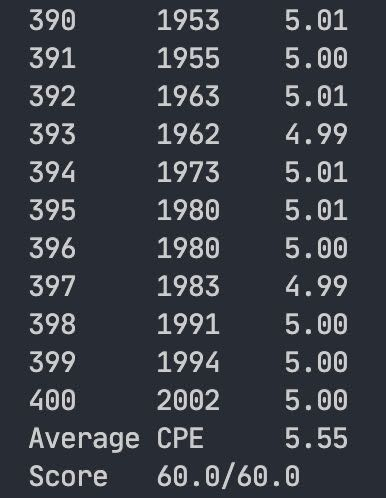
\includegraphics[width=0.4\textwidth]{partC-larger-scale-test.jpg} %插入图片,[]中设置图片大小,{}中是图片文件名
        \caption{partC larger scale test} %最终文档中希望显示的图片标题
        \label{Fig.partC-correctness} %用于文内引用的标签
\end{figure}
From analysis, we could safely estimate that the theoretical minimum $CPE$ should be around $5.0$. \\
\\
\textbf{So it's almost certain that the optimizations we've done under the existing ISA framework are close to extreme.}
\subsubsection{Code readability}
We put a lot of effort into the readability of the code for parts A.
\begin{itemize}
        \item For functions that contain loops, we can always break it down into three logical regions: "loop", "test", and "return".
        \item For various registers, we always annotate its purpose with comments
        \item For code that's not so obvious, we always leave the comment showing its counterpart in the C function next to it.
\end{itemize}
We have also left understandable and sufficient comments in the header of the modified files in partB and partC, 
please open ncopy.ys, pipe-zzcc.hcl, SEQ-full.hcl to read

\subsection{Feelings}
This is a very interesting and valuable project. Ziqi and I work together perfectly. 
When Ziqi achieved full score for partC in two hours, we started thinking about whether we could get CPE down to the limit of 5.
We ended up spending two days talking, drawing, and writing code to test.
But what was so exciting was that after two big failures, we finally got there in a very "weird" way.
It should be noted, however, that there is an inherent problem with the simulator for the pipeline processor, 
otherwise our attempt 2 should have been successful and would not have required special means to implement it.
This project allowed us to reap the valuable sense of accomplishment brought by not giving up. 
We are also very grateful to have been able to take this course and to be introduced to such a valuable project.
%----------------------------------------------------------------------------------------
\end{document}